%%%%%%%%%%%%%%%%%%%%%%%%%%%%%%%%%%%%%%%%%
% Structured General Purpose Assignment
% LaTeX Template
%
% This template has been downloaded from:
% http://www.latextemplates.com
%
% Original author:
% Ted Pavlic (http://www.tedpavlic.com)
%
% Note:
% The \lipsum[#] commands throughout this template generate dummy text
% to fill the template out. These commands should all be removed when 
% writing assignment content.
%
%%%%%%%%%%%%%%%%%%%%%%%%%%%%%%%%%%%%%%%%%


%----------------------------------------------------------------------------------------
%	PACKAGES AND OTHER DOCUMENT CONFIGURATIONS
%----------------------------------------------------------------------------------------

\documentclass{article}

%\usepackage{currfile}
\usepackage{fancyhdr} % Required for custom headers
\usepackage{lastpage} % Required to determine the last page for the footer
\usepackage{extramarks} % Required for headers and footers
\usepackage{graphicx} % Required to insert images
\usepackage{lipsum} % Used for inserting dummy 'Lorem ipsum' text into the template
\usepackage{outlines}
\usepackage{wrapfig}
\usepackage[dutch,]{babel}
\selectlanguage{dutch}
%
%%%\usepackage{pdfpages} % als we pdf willen includen --> pdflatex gebruiken

% Margins
\topmargin=-0.45in
\evensidemargin=0in
\oddsidemargin=0in
\textwidth=6.5in
\textheight=9.0in
\headsep=0.25in 

\linespread{1.1} % Line spacing

% Set up the header and footer
\pagestyle{fancy}
\lhead{\hmwkAuthorName} % Top left header
%\chead{\hmwkClass\ \small{(\textit{\hmwkClassInstructor})}} 
\chead{\hmwkClass} 
\rhead{\hmwkTitle} 
\lfoot{\LaTeX: \small{\input{filename.txt}}} % Bottom left footer
%\lfoot{\LaTeX: {/home/jan/CVOTSM/A7\_IT-organisatie/ITIL/}\currfilepath} % Bottom left footer
\cfoot{} % Bottom center footer
\rfoot{Pagina\ \thepage\ van\ \pageref{LastPage}} % Bottom right footer
\renewcommand\headrulewidth{0.4pt} % Size of the header rule
\renewcommand\footrulewidth{0.4pt} % Size of the footer rule

\setlength\parindent{0pt} % Removes all indentation from paragraphs


%\setlength{\parskip}{\baselineskip}%
%\setlength{\parindent}{12pt}%

%----------------------------------------------------------------------------------------
%	DOCUMENT STRUCTURE COMMANDS
%	Skip this unless you know what you're doing
%----------------------------------------------------------------------------------------

% Header and footer for when a page split occurs within a problem environment
\newcommand{\enterProblemHeader}[1]{
\nobreak\extramarks{#1}{#1 continued on next page\ldots}\nobreak
\nobreak\extramarks{#1 (continued)}{#1 continued on next page\ldots}\nobreak
}

% Header and footer for when a page split occurs between problem environments
\newcommand{\exitProblemHeader}[1]{
\nobreak\extramarks{#1 (continued)}{#1 continued on next page\ldots}\nobreak
\nobreak\extramarks{#1}{}\nobreak
}

\setcounter{secnumdepth}{0} % Removes default section numbers
\newcounter{homeworkProblemCounter} % Creates a counter to keep track of the number of problems

\newcommand{\homeworkProblemName}{}
\newenvironment{homeworkProblem}[1][Problem \arabic{homeworkProblemCounter}]{ % Makes a new environment called homeworkProblem which takes 1 argument (custom name) but the default is "Problem #"
\stepcounter{homeworkProblemCounter} % Increase counter for number of problems
\renewcommand{\homeworkProblemName}{#1} % Assign \homeworkProblemName the name of the problem
\section{\homeworkProblemName} % Make a section in the document with the custom problem count
\enterProblemHeader{\homeworkProblemName} % Header and footer within the environment
}{
\exitProblemHeader{\homeworkProblemName} % Header and footer after the environment
}

\newcommand{\problemAnswer}[1]{ % Defines the problem answer command with the content as the only argument
\noindent\framebox[\columnwidth][c]{\begin{minipage}{0.98\columnwidth}#1\end{minipage}} % Makes the box around the problem answer and puts the content inside
}

\newcommand{\homeworkSectionName}{}
\newenvironment{homeworkSection}[1]{ % New environment for sections within homework problems, takes 1 argument - the name of the section
\renewcommand{\homeworkSectionName}{#1} % Assign \homeworkSectionName to the name of the section from the environment argument
\subsection{\homeworkSectionName} % Make a subsection with the custom name of the subsection
\enterProblemHeader{\homeworkProblemName\ [\homeworkSectionName]} % Header and footer within the environment
}{
\enterProblemHeader{\homeworkProblemName} % Header and footer after the environment
}
   
%----------------------------------------------------------------------------------------
%	NAME AND CLASS SECTION
%----------------------------------------------------------------------------------------

\newcommand{\hmwkTitle}{10. Visueel Ontwerp} % Assignment title
%\newcommand{\hmwkDueDate}{Monday,\ January\ 1,\ 2012} % Due date
\newcommand{\hmwkDueDate}{} % Due date
\newcommand{\hmwkClass}{Projectwerk} % Course/class
%\newcommand{\hmwkClassTime}{10:30am} % Class/lecture time
\newcommand{\hmwkClassTime}{} % Class/lecture time
\newcommand{\hmwkClassInstructor}{} % Teacher/lecturer
\newcommand{\hmwkAuthorName}{Wagemakers Jan} % Your name

%----------------------------------------------------------------------------------------
%	TITLE PAGE
%----------------------------------------------------------------------------------------

\title{
\vspace{2in}
\textmd{\textbf{\hmwkClass}}\\
\textmd{\textbf{\hmwkTitle}}\\
%\normalsize\vspace{0.1in}\small{In\ te\ dienen\ voor\ \hmwkDueDate}\\
%\vspace{0.1in}{\textit{Leerkracht: \hmwkClassInstructor\ \hmwkClassTime}}
\vspace{3in}
}

\author{\textbf{\hmwkAuthorName}}
\date{\today} % Insert date here if you want it to appear below your name

%----------------------------------------------------------------------------------------

\begin{document}

\maketitle

%----------------------------------------------------------------------------------------
%	TABLE OF CONTENTS
%----------------------------------------------------------------------------------------

%\setcounter{tocdepth}{1} % Uncomment this line if you don't want subsections listed in the ToC

%\newpage
%\tableofcontents
\newpage

%%% Opdracht

%%%%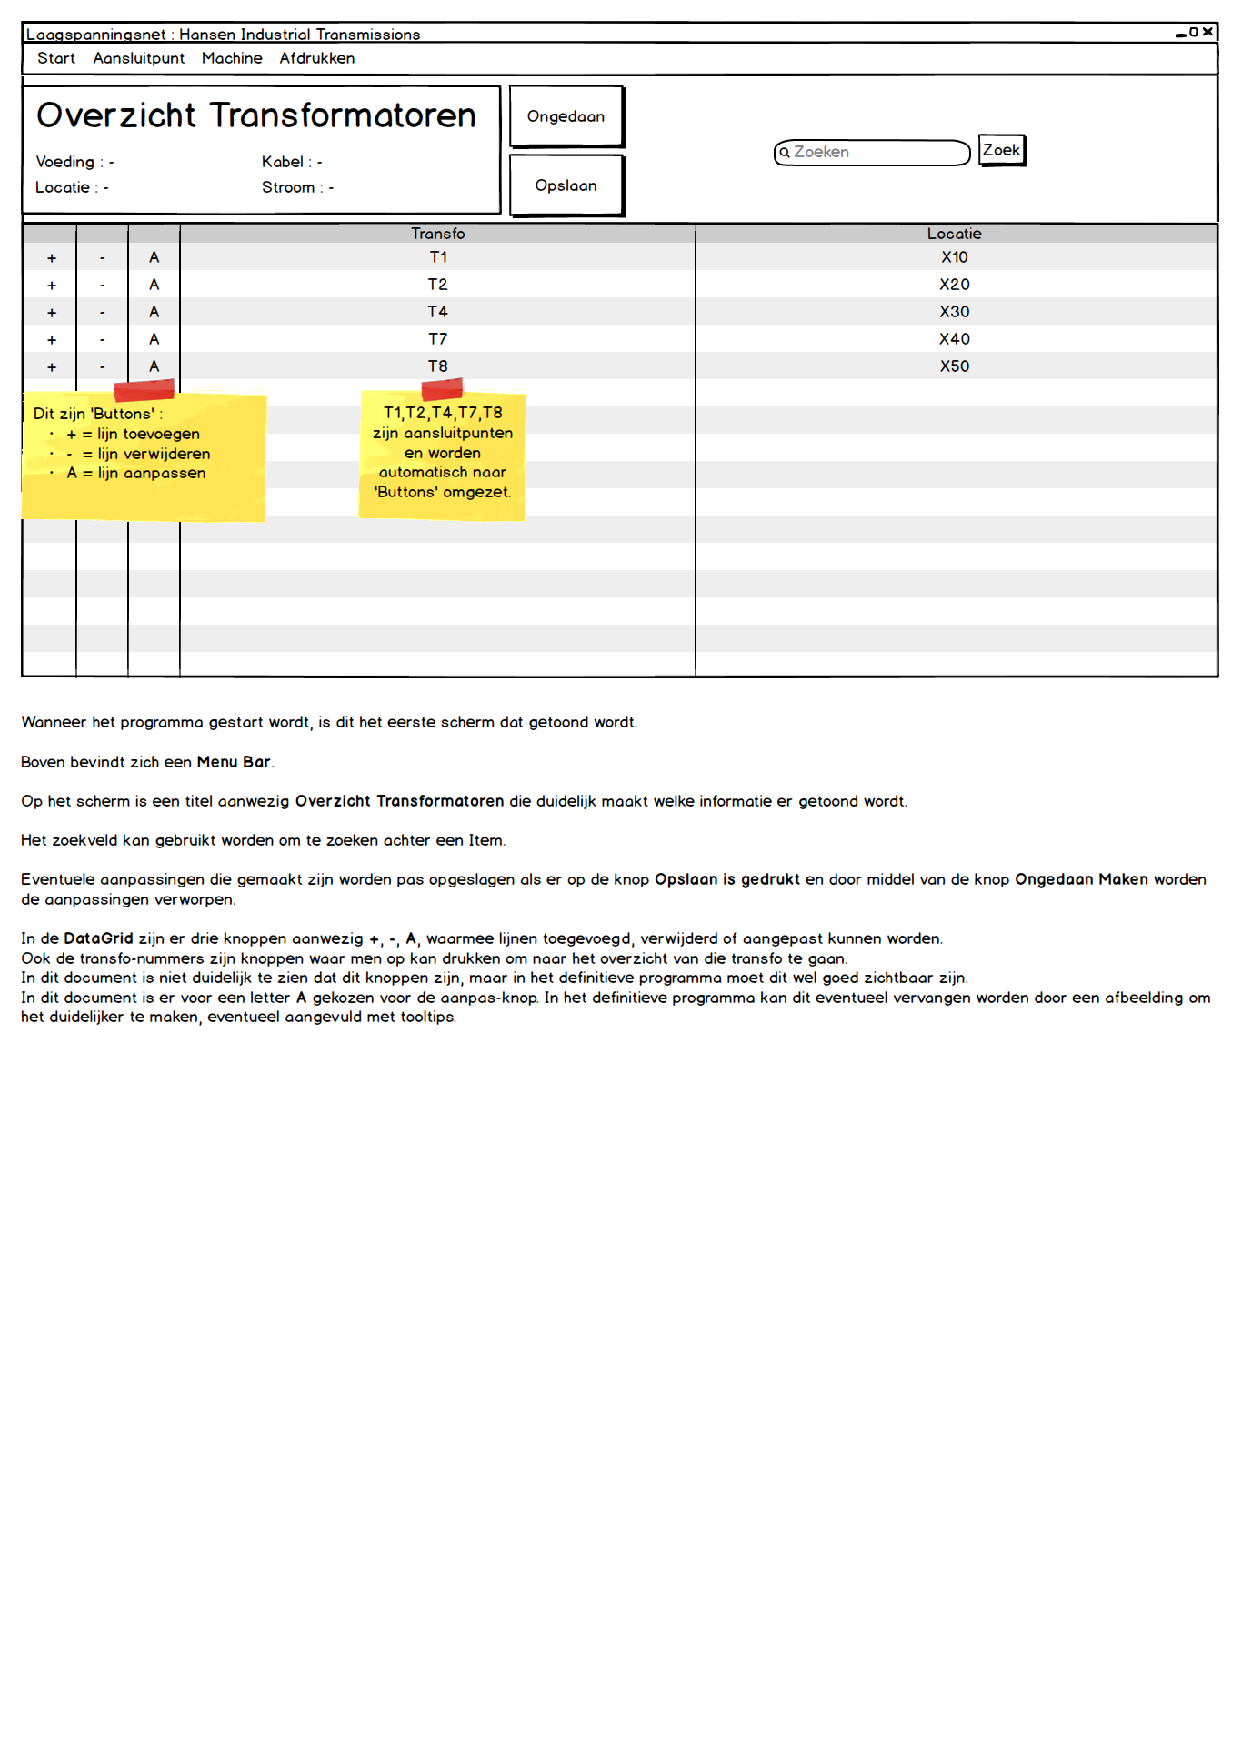
\includepdf[pages=-,scale=0.86,pagecommand={}]{/home/jan/MEGA/2017-2018/ProjectWerk/VisueelOntwerp.pdf}



%\begin{homeworkProblem}[\arabic{homeworkProblemCounter} : Omschrijving opdracht]
\begin{homeworkProblem}[Start]
\includegraphics[width=1\textwidth]{/home/jan/MEGA/2017-2018/ProjectWerk/Balsamiq/1.png}
\\\\
Wanneer het programma gestart wordt, is dit het eerste scherm dat getoond
wordt. 
\\\\
Boven bevindt zich een \textbf{Menu Bar}. Op het scherm is een titel
aanwezig \textbf{Overzicht Transformatoren} die duidelijk maakt welke
informatie er getoond wordt. Het \textbf{Zoekveld} kan gebruikt worden om te
zoeken naar een item. 
\\\\
Eventuele aanpassingen die gemaakt zijn worden pas
opgeslagen als er op de knop \textbf{Opslaan} is geklikt. Aanpassingen
worden verworpen door middel van de knop \textbf{Ongedaan maken}.
\\\\
In de \textbf{DataGrid} zijn er drie knoppen aanwezig \textbf{+},\textbf{-},
\textbf{A} waarmee lijnen toegevoegd, verwijderd of aangepast kunnen worden.
Ook de transfo-nummers zijn knoppen waar men op kan klikken om naar het
overzicht van die transfo te gaan. In dit document is niet duidelijk te zien
dat dit knoppen zijn, maar in het werkend programma moet dit wel goed
zichtbaar zijn. 
In dit document is er gekozen voor een
letter \textbf{A} voor de aanpas-knop. In het werkend programma kan dit
eventueel vervangen worden door een afbeelding (icoontje) om de functie
duidelijker te maken, eventueel aangevuld met tooltips.
\end{homeworkProblem}


\begin{homeworkProblem}[Layout transformator]
\includegraphics[width=1\textwidth]{/home/jan/MEGA/2017-2018/ProjectWerk/Balsamiq/2.png}
\\\\
Wanneer we in het overzicht van de transformatoren (zie vorig scherm) op een
transfo klikken, zal dit scherm getoond worden.
\\\\
De titel geeft aan dat de gegevens van transfo \textbf{T8} getoond worden.
Verder is het scherm gelijk aan het vorige scherm.
\\\\
Onder de titel \textbf{Layout van T8} is bij kabel, voeding, stroom geen
informatie aanwezig omdat voor transfo's deze informatie niet beschikbaar is
(dit programma beheert het laagspanningsnet, de voeding van transformatoren
is hoogspanning).
\end{homeworkProblem}

\begin{homeworkProblem}[Layout verdeelbord]
\includegraphics[width=1\textwidth]{/home/jan/MEGA/2017-2018/ProjectWerk/Balsamiq/3.png}
\\\\
Wanneer we in het overzicht van een tranformator (zie vorig scherm) op een
verdeelbord klikken, zal dit scherm getoond worden.
\\\\
De titel geeft aan dat de gegevens van verdeelbord \textbf{VB810} getoond worden.
Verder is het scherm gelijk aan het vorige scherm.
\\\\
Onder de titel \textbf{Layout van VB810} is bij kabel, voeding, stroom nu
wel informatie aanwezig.
\end{homeworkProblem}

\begin{homeworkProblem}[Layout zekeringkast]
\includegraphics[width=1\textwidth]{/home/jan/MEGA/2017-2018/ProjectWerk/Balsamiq/4.png}
\\\\
Wanneer we in het overzicht van een verdeelbord (zie vorig scherm) op een
(zekering-)kast klikken, zal dit scherm getoond worden.
\\\\
De titel geeft aan dat de gegevens van kast \textbf{K810a} getoond
worden.
Verder is het scherm gelijk aan het vorige scherm.
\\\\
Ook hier is onder de titel \textbf{Layout van K810a} de nodige informatie
bij kabel, voeding en stroom aanwezig.
\end{homeworkProblem}

\begin{homeworkProblem}[Aanpassen van een aansluiting]
\includegraphics[width=1\textwidth]{/home/jan/MEGA/2017-2018/ProjectWerk/Balsamiq/5.png}
\\\\
Door op de knop \textbf{A} te klikken zal een menu verschijnen waarmee we de
gegevens van die lijn kunnen aanpassen. Er verschijnt een nieuw scherm met
daarin de inhoud van die lijn. We kunnen kiezen of het al dan niet om een
\textbf{Machine},\textbf{Kast/Verdeelbord} gaat en alle gegevens aanpassen.
\end{homeworkProblem}

\begin{homeworkProblem}[Nieuwe Machine]
\includegraphics[width=1\textwidth]{/home/jan/MEGA/2017-2018/ProjectWerk/Balsamiq/6.png}
\\\\
Bij Machine kan er gekozen worden uit Machines die reeds in de database
zitten. Er kan ook \textbf{Geen} gekozen worden als het niet om een machine
gaat. Er kan ook gekozen worden om een nieuwe machine toe te voegen.
\end{homeworkProblem}

\begin{homeworkProblem}[Nieuwe Machine : ingeven]
\includegraphics[width=1\textwidth]{/home/jan/MEGA/2017-2018/ProjectWerk/Balsamiq/7.png}
\\\\
Als er gekozen wordt om een nieuwe machine in te geven, zal er een nieuw
venster verschijnen waar de nodige informatie ingevuld kan worden.
\end{homeworkProblem}

\begin{homeworkProblem}[Aanpassen van een aansluiting : Machine]
\includegraphics[width=1\textwidth]{/home/jan/MEGA/2017-2018/ProjectWerk/Balsamiq/8.png}
\\\\
Wanneer er bij het \textbf{aanpassen van een aansluiting} er voor een
\textbf{machine} gekozen
wordt (eventueel eerst aangemaakt zoals in vorig scherm), zal de
omschrijving uit de machine \textbf{table} van de database gehaald worden.
\\\\
\includegraphics[width=1\textwidth]{/home/jan/MEGA/2017-2018/ProjectWerk/Balsamiq/9.png}
\\\\
Ook de informatie over de kabel en de zekering (stroom) kan hier aangepast
worden.
\end{homeworkProblem}

\begin{homeworkProblem}[Aansluiting is aangepast]
\includegraphics[width=1\textwidth]{/home/jan/MEGA/2017-2018/ProjectWerk/Balsamiq/10.png}
\\\\
Wanneer de aangepaste gegevens zijn ingegeven, verschijnen deze in het
overzicht. De gegevens zijn echter nog niet opgeslagen. Door op de knop
\textbf{Opslaan} te klikken worden de gegevens opgenomen in de database.
Door op de knop \textbf{Ongedaan maken} te klikken zullen de vorige gegevens
terug getoond worden (database terug inlezen). De knoppen \textbf{Opslaan}
en \textbf{Ongedaan maken} kunnen het beste van kleur veranderen zodat
duidelijk te zien is wanneer er nog niet opgeslagen gegevens op het scherm
staan. Wanneer men van het scherm weg tracht te navigeren terwijl er nog
niet opgeslagen gegevens zijn zal dit aan de gebruiker gemeld worden.
\end{homeworkProblem}

\begin{homeworkProblem}[Een aansluiting leeg maken]
\includegraphics[width=1\textwidth]{/home/jan/MEGA/2017-2018/ProjectWerk/Balsamiq/11.png}
\\\\
Stel, er wordt een machine verwijderd en de desbetreffend aansluiting komt
vrij. We laten dan alle velden leeg die er niet toe doen. En klikken op
\textbf{OK}. De aansluiting is nu leeg.
\\\\
\includegraphics[width=1\textwidth]{/home/jan/MEGA/2017-2018/ProjectWerk/Balsamiq/12.png}
\end{homeworkProblem}

\begin{homeworkProblem}[Een verdeelbord aansluiten]
\includegraphics[width=1\textwidth]{/home/jan/MEGA/2017-2018/ProjectWerk/Balsamiq/13.png}
\\\\
Het aansluiten van een verdeelbord (of kast) werkt op analoge manier als het
aansluiten van een machine. Wel is het belangrijk om enige intelligentie
in het programma te steken om te bewaken dat de nummering consistent blijft.
\\\\
\includegraphics[width=1\textwidth]{/home/jan/MEGA/2017-2018/ProjectWerk/Balsamiq/14.png}
\end{homeworkProblem}

\begin{homeworkProblem}[Een nieuw verdeelbord]
\includegraphics[width=1\textwidth]{/home/jan/MEGA/2017-2018/ProjectWerk/Balsamiq/15.png}
\includegraphics[width=1\textwidth]{/home/jan/MEGA/2017-2018/ProjectWerk/Balsamiq/16.png}
\\\\
Op een analoge manier als een nieuwe machine aanmaken, kan er ook een nieuw
verdeelbord aangemaakt worden. 
\end{homeworkProblem}

\begin{homeworkProblem}[De + en - knoppen]
\includegraphics[width=1\textwidth]{/home/jan/MEGA/2017-2018/ProjectWerk/Balsamiq/17.png}
\\\\
Met de \textbf{+} knop kan er een lijn toegevoegd worden. Omdat na het
toevoegen van een lijn het logisch is dat deze van gegevens wordt voorzien,
zal na het toevoegen van een lijn automatisch het venster (zelfde venster
als bij \textbf{Aanpassen}) verschijnen om
deze lege lijn van informatie te voorzien.
\\\\
Met de \textbf{-} knop zal de lijn in kwestie verwijderd worden.
\\\\
Ook hier geldt dat deze aanpassingen pas in de database zullen opgenomen
worden als er op de knop \textbf{opslaan} is geklikt.
\end{homeworkProblem}

\begin{homeworkProblem}[Zoeken]
\includegraphics[width=1\textwidth]{/home/jan/MEGA/2017-2018/ProjectWerk/Balsamiq/18.png}
\\\\
Het \textbf{zoekveld} kan gebruikt worden om naar gegevens te zoeken. De
database zal volledig doorzocht worden en elke overeenkomst zal hier
verschijnen. Velden die in aanmerking komen om tijdens het zoeken gebruikt
te worden zijn omschrijving, en de nummers van machines,
kasten, verdeelborden, transfo's. Momenteel is er gekozen om dit niet op te
splitsen in meerdere zoekvelden omdat dit bij de gebruiker verwarring kan
veroorzaken. Als tijdens de testfase blijkt dat dit opsplitsen toch zinvol is
kan dit nog aangepast worden.
\\\\
Ook in de zoekresultaten worden aansluitpunten automatisch omgezet naar
knoppen om te kunnen navigeren naar dat aansluitpunt. 
\end{homeworkProblem}

\begin{homeworkProblem}[Menu : Start]
\includegraphics[width=1\textwidth]{/home/jan/MEGA/2017-2018/ProjectWerk/Balsamiq/19.png}
\\\\
Bovenaan het scherm bevindt zich een \textbf{MenuBar}. Door op start te
drukken zal men naar het \textbf{overzichtscherm van de transformatoren} springen.
\end{homeworkProblem}

\begin{homeworkProblem}[Menu : Aansluitpunt]
\includegraphics[width=1\textwidth]{/home/jan/MEGA/2017-2018/ProjectWerk/Balsamiq/20.png}
\\\\
Via het menu \textbf{Aansluitpunt} kunnen er aansluitpunten toegevoegd,
aangepast en verwijderd worden. De vensters om aansluitpunten aan te passen
of toe te voegen zijn dezelfde als die we eerder in het document gezien
hebben bij het aanpassen van een \textbf{aansluiting}.
\\\\
Bij het kiezen voor het verwijderen van een aansluitpunt zal een venster
verschijnen waar het te verwijderen aansluitpunt gekozen kan worden.
\end{homeworkProblem}

\begin{homeworkProblem}[Menu : Machine]
\includegraphics[width=1\textwidth]{/home/jan/MEGA/2017-2018/ProjectWerk/Balsamiq/21.png}
\\\\
Via het menu \textbf{Machine} kunnen er machines toegevoegd, aangepast en
verwijderd worden. De vensters om Machines aan te passen
of toe te voegen zijn dezelfde als die we eerder in het document gezien 
hebben bij het aanpassen van een \textbf{aansluiting}.
\\\\
Bij het kiezen voor het verwijderen van een machine zal een venster
verschijnen waar de te verwijderen machine gekozen kan worden.
\end{homeworkProblem}

\begin{homeworkProblem}[Menu : Afdrukken]
\includegraphics[width=1\textwidth]{/home/jan/MEGA/2017-2018/ProjectWerk/Balsamiq/22.png}
\\\\
Via het menu \textbf{Afdrukken} kunnen de gegevens afgedrukt worden. 
\\\\
Als men voor \textbf{Huidige pagina} kiest zullen de gegevens afgedrukt
worden die momenteel op het scherm zichtbaar zijn. Er zal onmiddelijk naar
de standaard printer afgedrukt worden, zonder dat er een scherm verschijnt.
Hierdoor kunnen gegevens snel afgedrukt worden.
\\\\
Als er meerdere gegevens afgedrukt dienen te worden kan dit via
\textbf{Afdrukken} $\rightarrow$ \textbf{Selectie}. Er zal dan een venster
verschijnen waar de printer, aantal kopie\"en en af te drukken gegevens
geselecteerd kunnen worden. Door \textbf{inclusief aansluitingen} aan te
vinken zullen de gegevens van aangesloten aansluitpunten ook afgedrukt
worden. Bv. \textbf{VB810} inclusief aansluitpunten $= VB810 + K810a +
K810b$. Ook hier kan men selecteren om de \textbf{huidige pagina} af te
drukken, zinvol als men deze via een niet standaard printer wil
afdrukken.
\end{homeworkProblem}

\begin{homeworkProblem}[Meldingen]
\includegraphics[width=1\textwidth]{/home/jan/MEGA/2017-2018/ProjectWerk/Balsamiq/23.png}
\\\\
Tijdens het uitvoeren van het programma kan het nodig zijn om de gebruiker
\textbf{meldingen} te geven. Meldingen kunnen zijn :

\begin{itemize}  
\item Toevoegen van een Machine of Aansluitpunt dat reeds bestaat. 
\item Verwijderen ven een Machine of Aansluitpunt dat nog in gebruik is.
\item Connectie problemen met de database server
\item \ldots 
\end{itemize}
\end{homeworkProblem}

% ==========================================================================================================================================

\end{document}
